\chapter{插值 POD 方法}
\label{cha:sysu-thesis-latex-install-guide}
POD方法在流场计算的应用,通常都是将流动方程投影在POD基上,获得低阶非线性方程,该方法已用于翼型的优化设计及多学科优化设计。近年来,插值POD方法被提出,并用于求流场近似解。

\section{插值POD方法}
POD 方法的采样解都是对实际问题中的某一或者某几个物理量进行一系列有规律的扰动得来的。在流体力学中扰动变量可以是时间、迎角、马赫数、翼型的几何外形甚至是多个扰动变量。由这些采样解求得的 POD 基可以表示该物理量扰动范围内的任意情况下的物理解。根据公式(2-2),每个解都对应一组基系数,采样解也同样对应一组基系数。若扰动变量与基系数之间存在连续的函数关系,则可以根据三次样条插值,利用采样解的扰动变量与基系数,求得扰动范围内的任意扰动情况下的物理解。设有 \(n\) 个扰动变量,每个扰动变量变化 \(m\) 次,计算过程如下:
\begin{enumerate}
    \item 确定扰动变量 \(\delta_j^{(i)}\)(\(j = 1, 2, \ldots, n\)),并由该扰动变量获得一组采样解 \(\{\mathbf{U}_i\}_{i=1}^m\);
    \item 由采样解 \(\{\mathbf{U}_i\}_{i=1}^m\) 计算 POD 基 \(\{\Phi^i\}_{i=1}^m\);
    \item 用所求的基表达采样解,一般使用一部分基就可以获得很好的表达效果:\(\mathbf{U}^i = \sum_{j=1}^r \alpha_j^i \Phi^j\)(\(p < m \times n\)),对应的基系数可由下式求得:\(\alpha_j^i = (\Phi^j, \mathbf{U}^i)\);
    \item 如果 \(\{\alpha_j^i\}_{i=1}^m\)(\(j = 1, 2, \ldots, p\))是扰动变量 \(\{\delta_j^i\}_{i=1}^m\)(\(j = 1, 2, \ldots, n\))的连续的函数,则可以利用三次样条插值求得不包括在采样解扰动变量里的任意一个扰动变量 \(\delta_j\) 所对应的基系数 \(\alpha_j^i\)。对应的物理解可以表示为:\(\mathbf{U}^i = \sum_{j=1}^r \alpha_j^i \Phi^j\)。
\end{enumerate}

\section{单变量三次样条插值方法}
\subsection{数学描述}
考虑定义在区间$[a,b]$上的三次样条插值问题。给定节点$\{x_0,x_1,...,x_n\}$及其对应函数值$\{f(x_i)\}$,要求构造分段三次多项式函数$S(x)$满足:

\begin{enumerate}
    \item 在子区间$[x_i, x_{i+1}]$上的局部表达式为:
    \begin{equation}
        S_i(x) = a_i + b_i(x-x_i) + c_i(x-x_i)^2 + d_i(x-x_i)^3
    \end{equation}
    
    \item 整体满足$C^2$连续性:
    \begin{align}
        \lim_{x\to x_i^+} S^{(k)}(x) &= \lim_{x\to x_i^-} S^{(k)}(x), \quad k=0,1,2
    \end{align}
    
    \item 自然边界条件:
    \begin{equation}
        S''(x_0) = S''(x_n) = 0
    \end{equation}
\end{enumerate}

\subsection{系数求解}
令$M_i = S''(x_i)$,根据三次多项式的二阶导数特性,可得递推关系:
\begin{equation}
    \frac{h_{i-1}}{6}M_{i-1} + \frac{h_{i-1}+h_i}{3}M_i + \frac{h_i}{6}M_{i+1} = \frac{f(x_{i+1})-f(x_i)}{h_i} - \frac{f(x_i)-f(x_{i-1})}{h_{i-1}}
\end{equation}

其中$h_i = x_{i+1}-x_i$。该方程组可表示为三对角矩阵形式:
\begin{equation}
    \begin{pmatrix}
        2 & \lambda_1 & 0 & \cdots & 0 \\
        \mu_2 & 2 & \lambda_2 & \cdots & 0 \\
        \vdots & \ddots & \ddots & \ddots & \vdots \\
        0 & \cdots & \mu_{n-1} & 2 & \lambda_{n-1} \\
        0 & \cdots & 0 & \mu_n & 2
    \end{pmatrix}
    \begin{pmatrix}
        M_1 \\ M_2 \\ \vdots \\ M_{n-1} \\ M_n
    \end{pmatrix}
    = \mathbf{b}
\end{equation}

其中$\mu_i = h_{i-1}/(h_{i-1}+h_i)$,$\lambda_i = 1-\mu_i$,右端项$\mathbf{b}$由差商计算。通过Thomas算法可高效求解该方程组。

\section{双变量三次样条插值方法}
\subsection{数学描述}
对于定义在矩形区域$[a,b]\times[c,d]$上的双变量插值问题,给定网格节点$\{(x_i,y_j)\}$及其对应函数值$\{f(x_i,y_j)\}$,构造双三次样条函数$S(x,y)$满足:

\begin{enumerate}
    \item 在子区域$[x_i,x_{i+1}]\times[y_j,y_{j+1}]$上的局部表达式为:
    \begin{equation}
        S_{ij}(x,y) = \sum_{k=0}^3\sum_{l=0}^3 \alpha_{kl}^{(ij)}(x-x_i)^k(y-y_j)^l
    \end{equation}
    
    \item 整体满足$C^1$连续性:
    \begin{align}
        \frac{\partial S_{ij}}{\partial x}(x_{i+1},y) &= \frac{\partial S_{i+1,j}}{\partial x}(x_{i+1},y) \\
        \frac{\partial S_{ij}}{\partial y}(x,y_{j+1}) &= \frac{\partial S_{i,j+1}}{\partial y}(x,y_{j+1})
    \end{align}
\end{enumerate}

\subsection{系数求解}
利用Hermite插值条件,每个节点的16个参数由以下条件确定:
\begin{equation}
    \begin{cases}
        S(x_i,y_j) = f(x_i,y_j) \\
        \frac{\partial S}{\partial x}(x_i,y_j) = f_x(x_i,y_j) \\
        \frac{\partial S}{\partial y}(x_i,y_j) = f_y(x_i,y_j) \\
        \frac{\partial^2 S}{\partial x\partial y}(x_i,y_j) = f_{xy}(x_i,y_j)
    \end{cases}
\end{equation}

通过联立相邻子区域的连续性条件,最终形成稀疏线性方程组:
其中$\mathbf{K}$为分块带状矩阵,$\boldsymbol{\alpha}$包含所有子区域的Bézier系数,$\mathbf{F}$由节点处的函数值和导数值构成。
\begin{equation}
    \mathbf{K}\boldsymbol{\alpha} = \mathbf{F}
\end{equation}
式3.10可展开为:
\begin{equation}
\underbrace{
\begin{pmatrix}
\mathbf{K}_{11} & \mathbf{K}_{12} & \cdots & \mathbf{K}_{1N} \\
\mathbf{K}_{21} & \mathbf{K}_{22} & \cdots & \mathbf{K}_{2N} \\
\vdots & \vdots & \ddots & \vdots \\
\mathbf{K}_{M1} & \mathbf{K}_{M2} & \cdots & \mathbf{K}_{MN}
\end{pmatrix}
}_{\mathbf{K}}
\underbrace{
\begin{pmatrix}
\boldsymbol{\alpha}^{(11)} \\
\boldsymbol{\alpha}^{(12)} \\
\vdots \\
\boldsymbol{\alpha}^{(mn)}
\end{pmatrix}
}_{\boldsymbol{\alpha}}
=
\underbrace{
\begin{pmatrix}
\mathbf{F}^{(11)} \\
\mathbf{F}^{(12)} \\
\vdots \\
\mathbf{F}^{(mn)}
\end{pmatrix}
}_{\mathbf{F}}
\end{equation}

其中:
\begin{itemize}
    \item 每个子矩阵$\mathbf{K}_{ij} \in \mathbb{R}^{16 \times 16}$对应子区域$[x_i,x_{i+1}]\times[y_j,y_{j+1}]$的系数约束,包含以下元素:
    \[
    \mathbf{K}_{ij}(p,q) = \frac{\partial \Phi_p}{\partial x^{k}\partial y^{l}}(x_i,y_j), \quad k+l \leq 2
    \]
    其中$\Phi_p$为双三次基函数,$p,q=1,...,16$。

    \item 向量$\boldsymbol{\alpha}^{(ij)} = (\alpha_{00}^{(ij)},...,\alpha_{33}^{(ij)})^\top$包含子区域$(i,j)$的16个多项式系数。

    \item 右端项$\mathbf{F}^{(ij)} \in \mathbb{R}^{16}$包含节点$(x_i,y_j)$的插值条件:
    \[
    \mathbf{F}^{(ij)} = \left(f(x_i,y_j),\ \frac{\partial f}{\partial x}\bigg|_{(x_i,y_j)},\ \frac{\partial f}{\partial y}\bigg|_{(x_i,y_j)},\ \frac{\partial^2 f}{\partial x\partial y}\bigg|_{(x_i,y_j)},\ 0,\ ...,\ 0\right)^\top
    \]
\end{itemize}

非对角块$\mathbf{K}_{i\neq j}$包含相邻子区域间的$C^1$连续性条件:
\[
\begin{cases}
\sum_{k=0}^3\sum_{l=0}^3 \alpha_{kl}^{(ij)} \cdot k \cdot x_{\mathrm{boundary}}^{k-1} y^l = \sum_{k=0}^3\sum_{l=0}^3 \alpha_{kl}^{(i+1,j)} \cdot k \cdot 0^{k-1} y^l & \text{(横向连续性)} \\
\sum_{k=0}^3\sum_{l=0}^3 \alpha_{kl}^{(ij)} \cdot l \cdot x^k y_{\mathrm{boundary}}^{l-1} = \sum_{k=0}^3\sum_{l=0}^3 \alpha_{kl}^{(i,j+1)} \cdot l \cdot x^k 0^{l-1} & \text{(纵向连续性)}
\end{cases}
\]


\section{Kriging 模型理论}
\subsection{Kriging 函数模型}

Kriging 函数模型由回归模型与相关模型相加而成,其形式为:
\begin{equation}
    y(x) = f(x)^T \beta + z(x)
    \label{eq:2.1}
\end{equation}
式中:\( f(x) \) 为多项式模型(回归模型),根据需求可以选择零阶、一阶、二阶多项式,其表达式为:
\begin{equation}
    f(x)^T \beta = [f_1(x), f_2(x), \ldots, f_p(x)] \beta = f_1(x) \beta_1 + f_2(x) \beta_2 + \cdots + f_p(x) \beta_p
    \label{eq:2.2}
\end{equation}
式中:

\( p \) —— 多项式数量;\\
\( \beta \) —— 线性回归系数的向量;\\
\( z(x) \) —— 被假定为遵循 \( (0, \sigma^2) \) 正态分布,且数学期望为 0、标准偏差为 \( \sigma \) 的随机过程(相关模型)。

\subsection{二阶平稳假定}
(1)随机过程 \( z(x) \) 的数学期望是一个确定的常数:
\begin{equation}
    E[z(x)] = a
    \label{eq:2.3}
\end{equation}
(2)区域化变量 \( z(x) \) 的协方差函数存在并且相等:
\begin{align}
    Cov[z(x), z(x+h)] &= E[(z(x) - E[z(x)])(z(x+h) - E[z(x+h)])] \notag \\
    &= E[z(x)z(x+h)] - E[z(x)]E[z(x+h)] \notag \\
    &= E[z(x)z(x+h)] - a^2 \notag \\
    &= Cov(h)
    \label{eq:2.4}
\end{align}
区域化变量 \( z(x) \) 的协方差矩阵为:
\begin{equation}
    Cov[z(x_i), z(x_j)] = \sigma^2 R[R(x_i, x_j)]
    \label{eq:2.5}
\end{equation}
式中:\( R \) —— 相关矩阵,其函数形式见表2.1;\\
\( R(x_i, x_j) \) —— 两个样本点 \( x_i, x_j \) 之间的空间相关函数。
\begin{table}[htbp]
    \centering
    \caption{相关矩阵 \( R(x_i, x_j) \) 的函数形式}
    \label{tab:2.1}
    \begin{tabular}{ll}
        \toprule
        相关函数 & \( R(x_i, x_j) \) \\
        \midrule
        高阶函数 & \( \exp(-\theta_j|d_i|) \) \\
        指数函数 & \( \exp(-\theta_j|d_i|) \) \\
        线性函数 & \( \max\{0, 1 - \theta_j|d_i|\} \) \\
        球形函数 & \( 1 - 1.5\xi_i + 0.5\xi_j^3 \) \\
        三次函数 & \( 1 - 3\xi_j + 2\xi_j^2 \) \\
        样本函数 & 
        \( \begin{cases}
            1 - 1.5\xi_i + 30\xi_j^3, & 0 \leq \xi_i \leq 0.2 \\
            1.25(1 - \xi_i)^2, & 0.2 < \xi_i < 1 
        \end{cases} \) \\
        \bottomrule
    \end{tabular}
\end{table}

注:1. 表中 \( d_i = |x_i - x_j| \),\( x_i \) 分别为两个样本点的第 \( n \) 个分量;\\
2. \( \theta_j \) 为特征值参数,控制不同维度上相关性的概率。
样本的似然函数表达式为:
\begin{equation}
    L = \frac{1}{(2\pi\sigma^2)^{n/2}|R|^{1/2}} \exp\left[-\frac{(Y-F\beta)^T R^{-1}(Y-F\beta)}{2\sigma^2}\right]
    \label{eq:2.7}
\end{equation}
通过最大似然估计可得:
\begin{align}
    \hat{\beta} &= (F^T R^{-1} F)^{-1} F^T R^{-1} Y
    \label{eq:2.8} \\
    \hat{\sigma}^2 &= \frac{(Y-F\hat{\beta})^T R^{-1} (Y-F\hat{\beta})}{n}
    \label{eq:2.9} \\
    \ln(\mathcal{L}) &= -\frac{n}{2} \ln(\hat{\sigma}^2) - \frac{1}{2} \ln |R|
    \label{eq:2.10}
\end{align}
未知点响应预测值为:
\begin{equation}
    \hat{y}(x_0) = f(x_0)^T \hat{\beta} + r(x_0)^T R^{-1} (Y-F\hat{\beta})
    \label{eq:2.11}
\end{equation}
预测值的方差为:
\begin{equation}
    \hat{\sigma}^2(x) = \sigma^2 \left[ 1 - \begin{pmatrix} f(x)^T & r(x)^T \end{pmatrix} \begin{pmatrix} 0 & F^T \\ R & r(x) \end{pmatrix}^{-1} \begin{pmatrix} f(x) \\ r(x) \end{pmatrix} \right]
    \label{eq:2.12}
\end{equation}
当预测第\( i \)个样本点时,有:
\begin{equation}
    \hat{y}(x_i) = f(x_i)^T \hat{\beta} + y_i - f(x_i)^T \hat{\beta} = y_i
    \label{eq:2.14}
\end{equation}
\section{数据对比分析方法}
\label{sec:4.1}
为系统评估插值POD方法的流场重构性能,本研究采用定量误差分析与相关性验证相结合的评价体系。具体通过以下三类指标实现:

\begin{itemize}
    \item {均方根误差(RMSE)}:反映局部大误差分布特征
    \begin{equation}
        \text{RMSE} = \sqrt{\frac{1}{n} \sum_{i=1}^{n} \left( y_i^{\text{pred}} - y_i^{\text{true}} \right)^2}
        \label{eq:rmse}
    \end{equation}

    \item{平均绝对误差(MAE)}:表征全局误差水平
    \begin{equation}
        \text{MAE} = \frac{1}{n} \sum_{i=1}^{n} \left| y_i^{\text{pred}} - y_i^{\text{true}} \right|
        \label{eq:mae}
    \end{equation}

    \item{皮尔逊相关系数(Pearson's $r$)}:评估趋势一致性
    \begin{equation}
        r = \frac{\sum_{i=1}^{n} (y_i^{\text{pred}} - \bar{y}^{\text{pred}})(y_i^{\text{true}} - \bar{y}^{\text{true}})}
        {\sqrt{\sum_{i=1}^{n} (y_i^{\text{pred}} - \bar{y}^{\text{pred}})^2 \sum_{i=1}^{n} (y_i^{\text{true}} - \bar{y}^{\text{true}})^2}}
        \label{eq:pearson}
    \end{equation}
\end{itemize}

%缺少两个图片

% Overleaf\footnote{网址可见\url{https://www.overleaf.com/}}是一个在线的Latex文档协作平台。我们不需要配置任何环境,便能够在上面直接使用本模板进行写作。操作步骤如下:

% 第一步,下载本项目压缩包(从\url{https://github.com/SYSU-SCC/sysu-thesis/releases}处下载即可),注意需要下载zip格式的压缩包。
% 然后,我们在Overleaf上新建项目,并上传该压缩包,可参考\autoref{fig:overleaf-new-proj}。


% \begin{figure}[h]
% 	\centering
% 	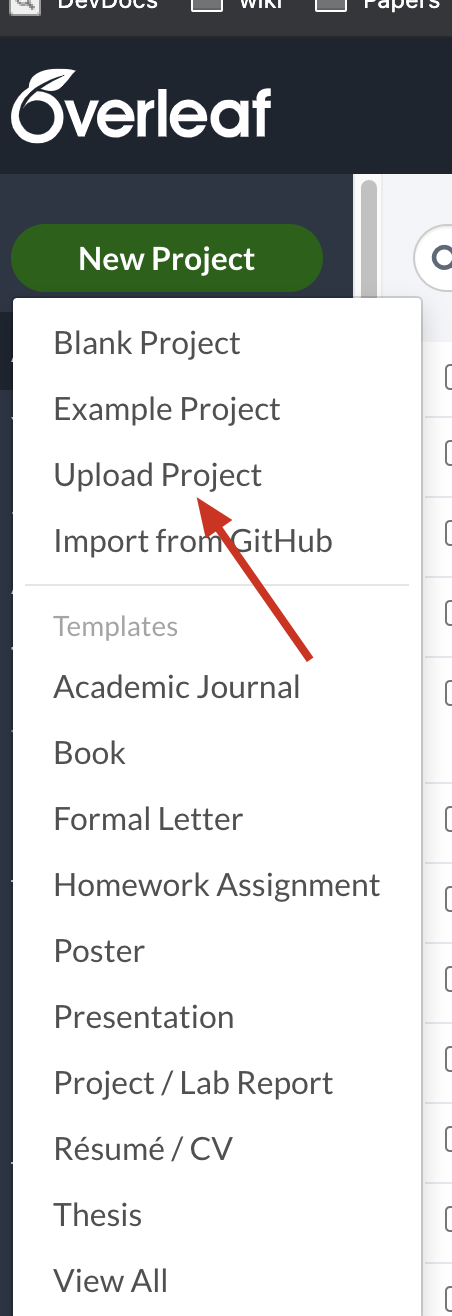
\includegraphics[width=0.2\textwidth]{image/chap03/overleaf-create-proj.jpg}
% 	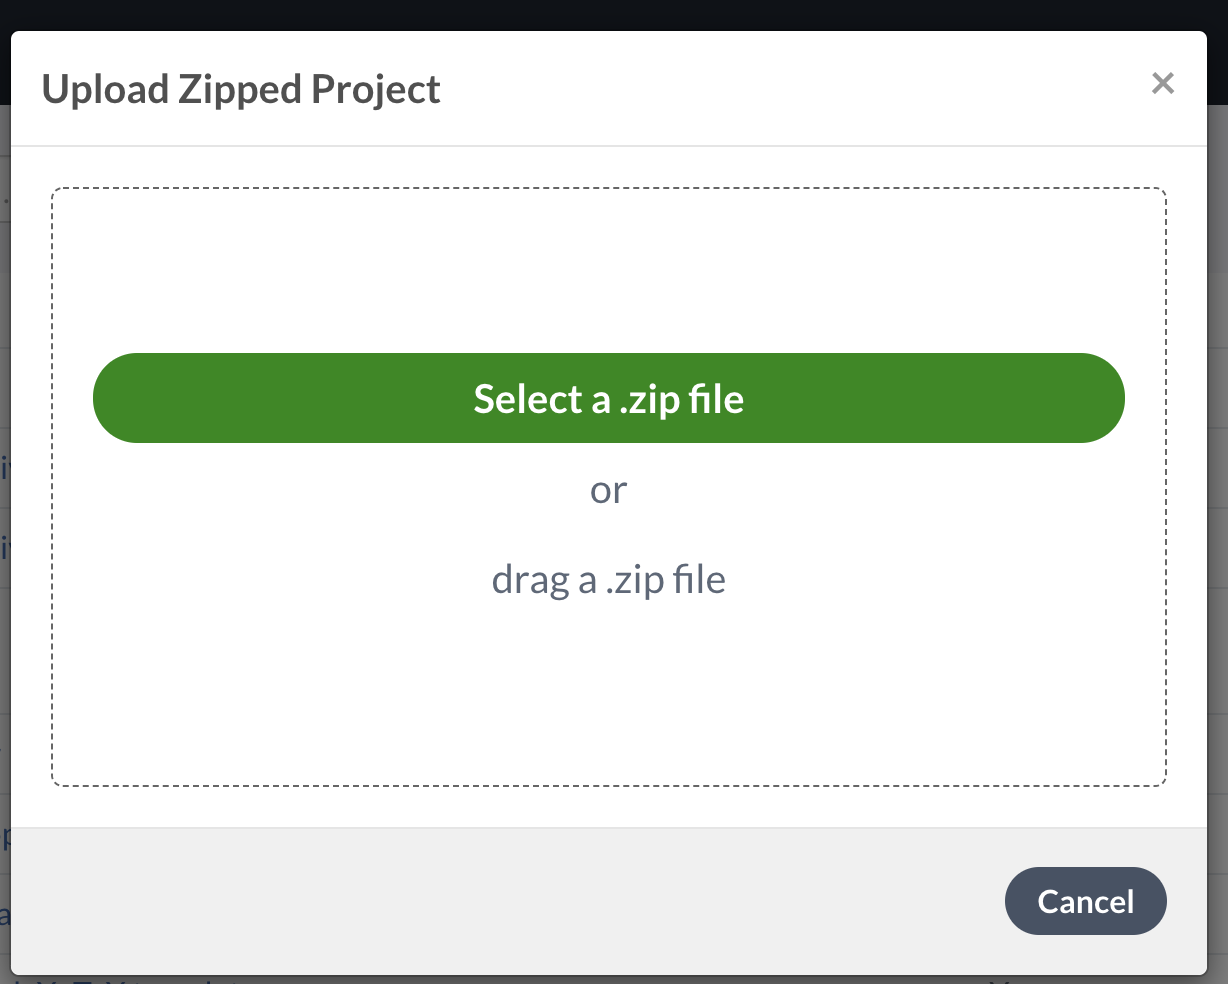
\includegraphics[width=0.7\textwidth]{image/chap03/overleaf-upload-proj.jpg}
% 	\caption{在Overleaf上创建并上传压缩包。}
% 	\label{fig:overleaf-new-proj}
% \end{figure}

% 第二步,在Overleaf的菜单中调整编译工具为\texttt{xelatex},可参考\autoref{fig:overleaf-config}。

% \begin{figure}[h]
% 	\centering
% 	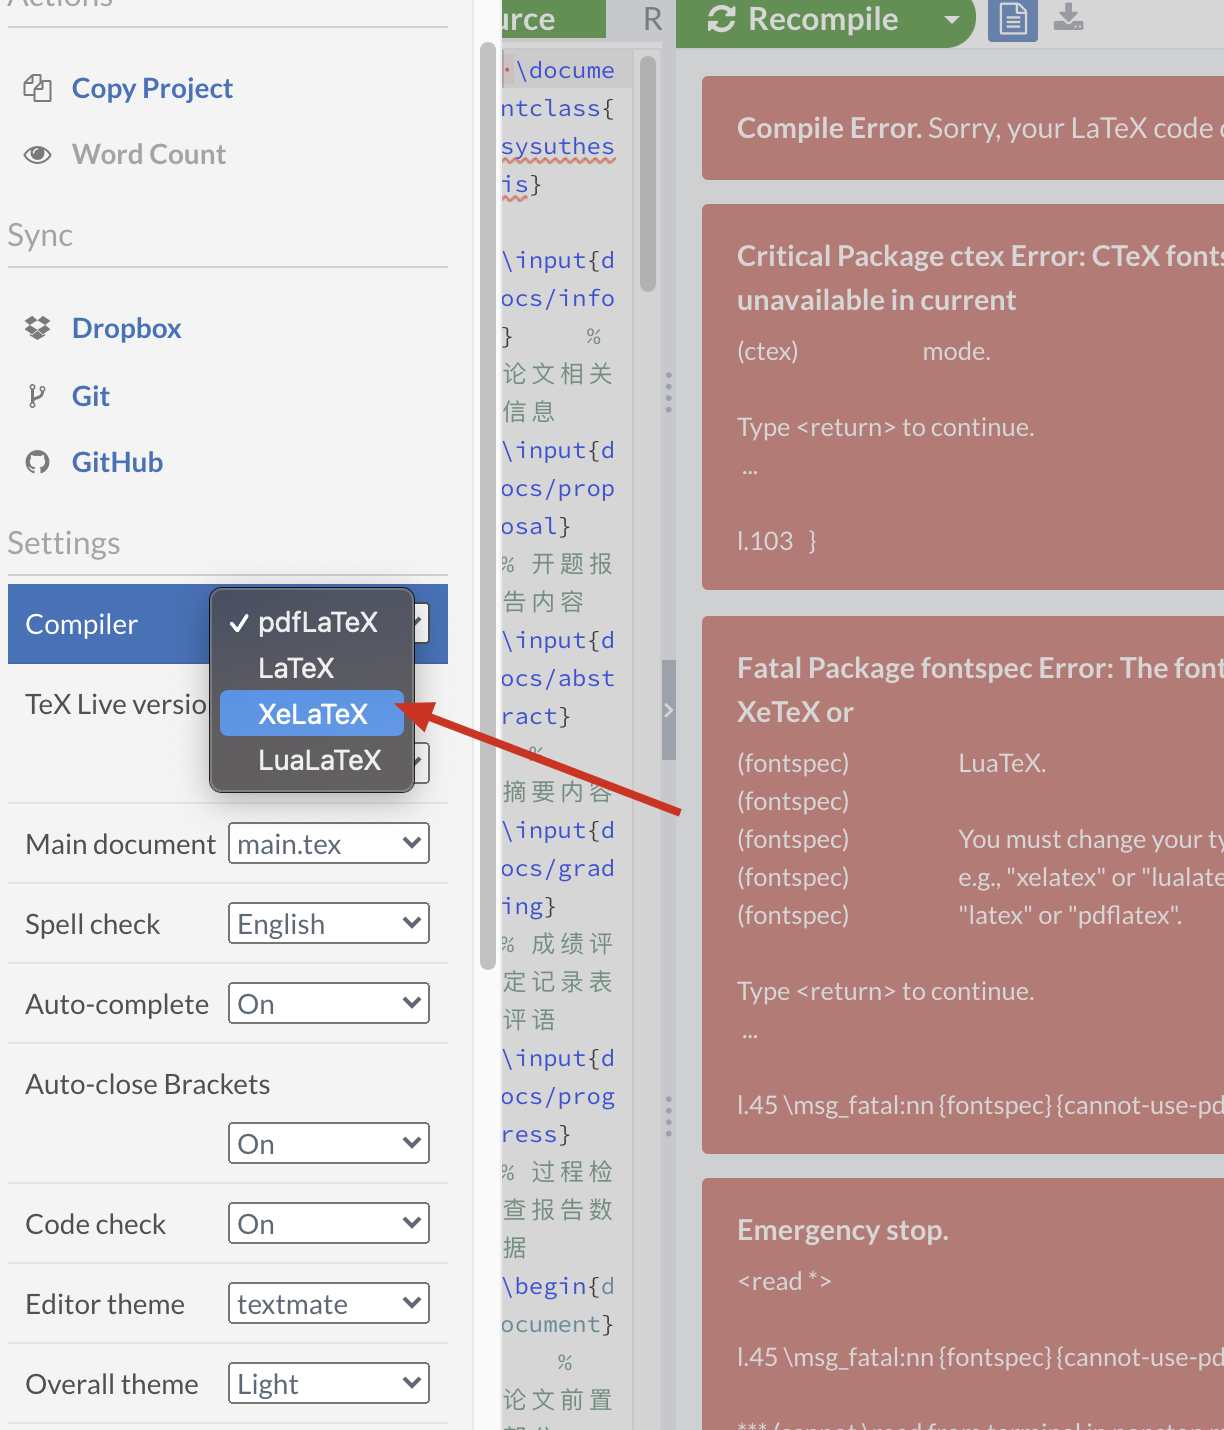
\includegraphics[width=0.6\textwidth]{image/chap03/overleaf-config.jpg}
% 	\caption{在Overleaf上调整编译工具}
% 	\label{fig:overleaf-config}
% \end{figure}


% 第三步,点击编译,得到本pdf,可以开始修改pdf了!最终可见\autoref{fig:overleaf-example}。


% \begin{figure}[h]
% 	\centering
% 	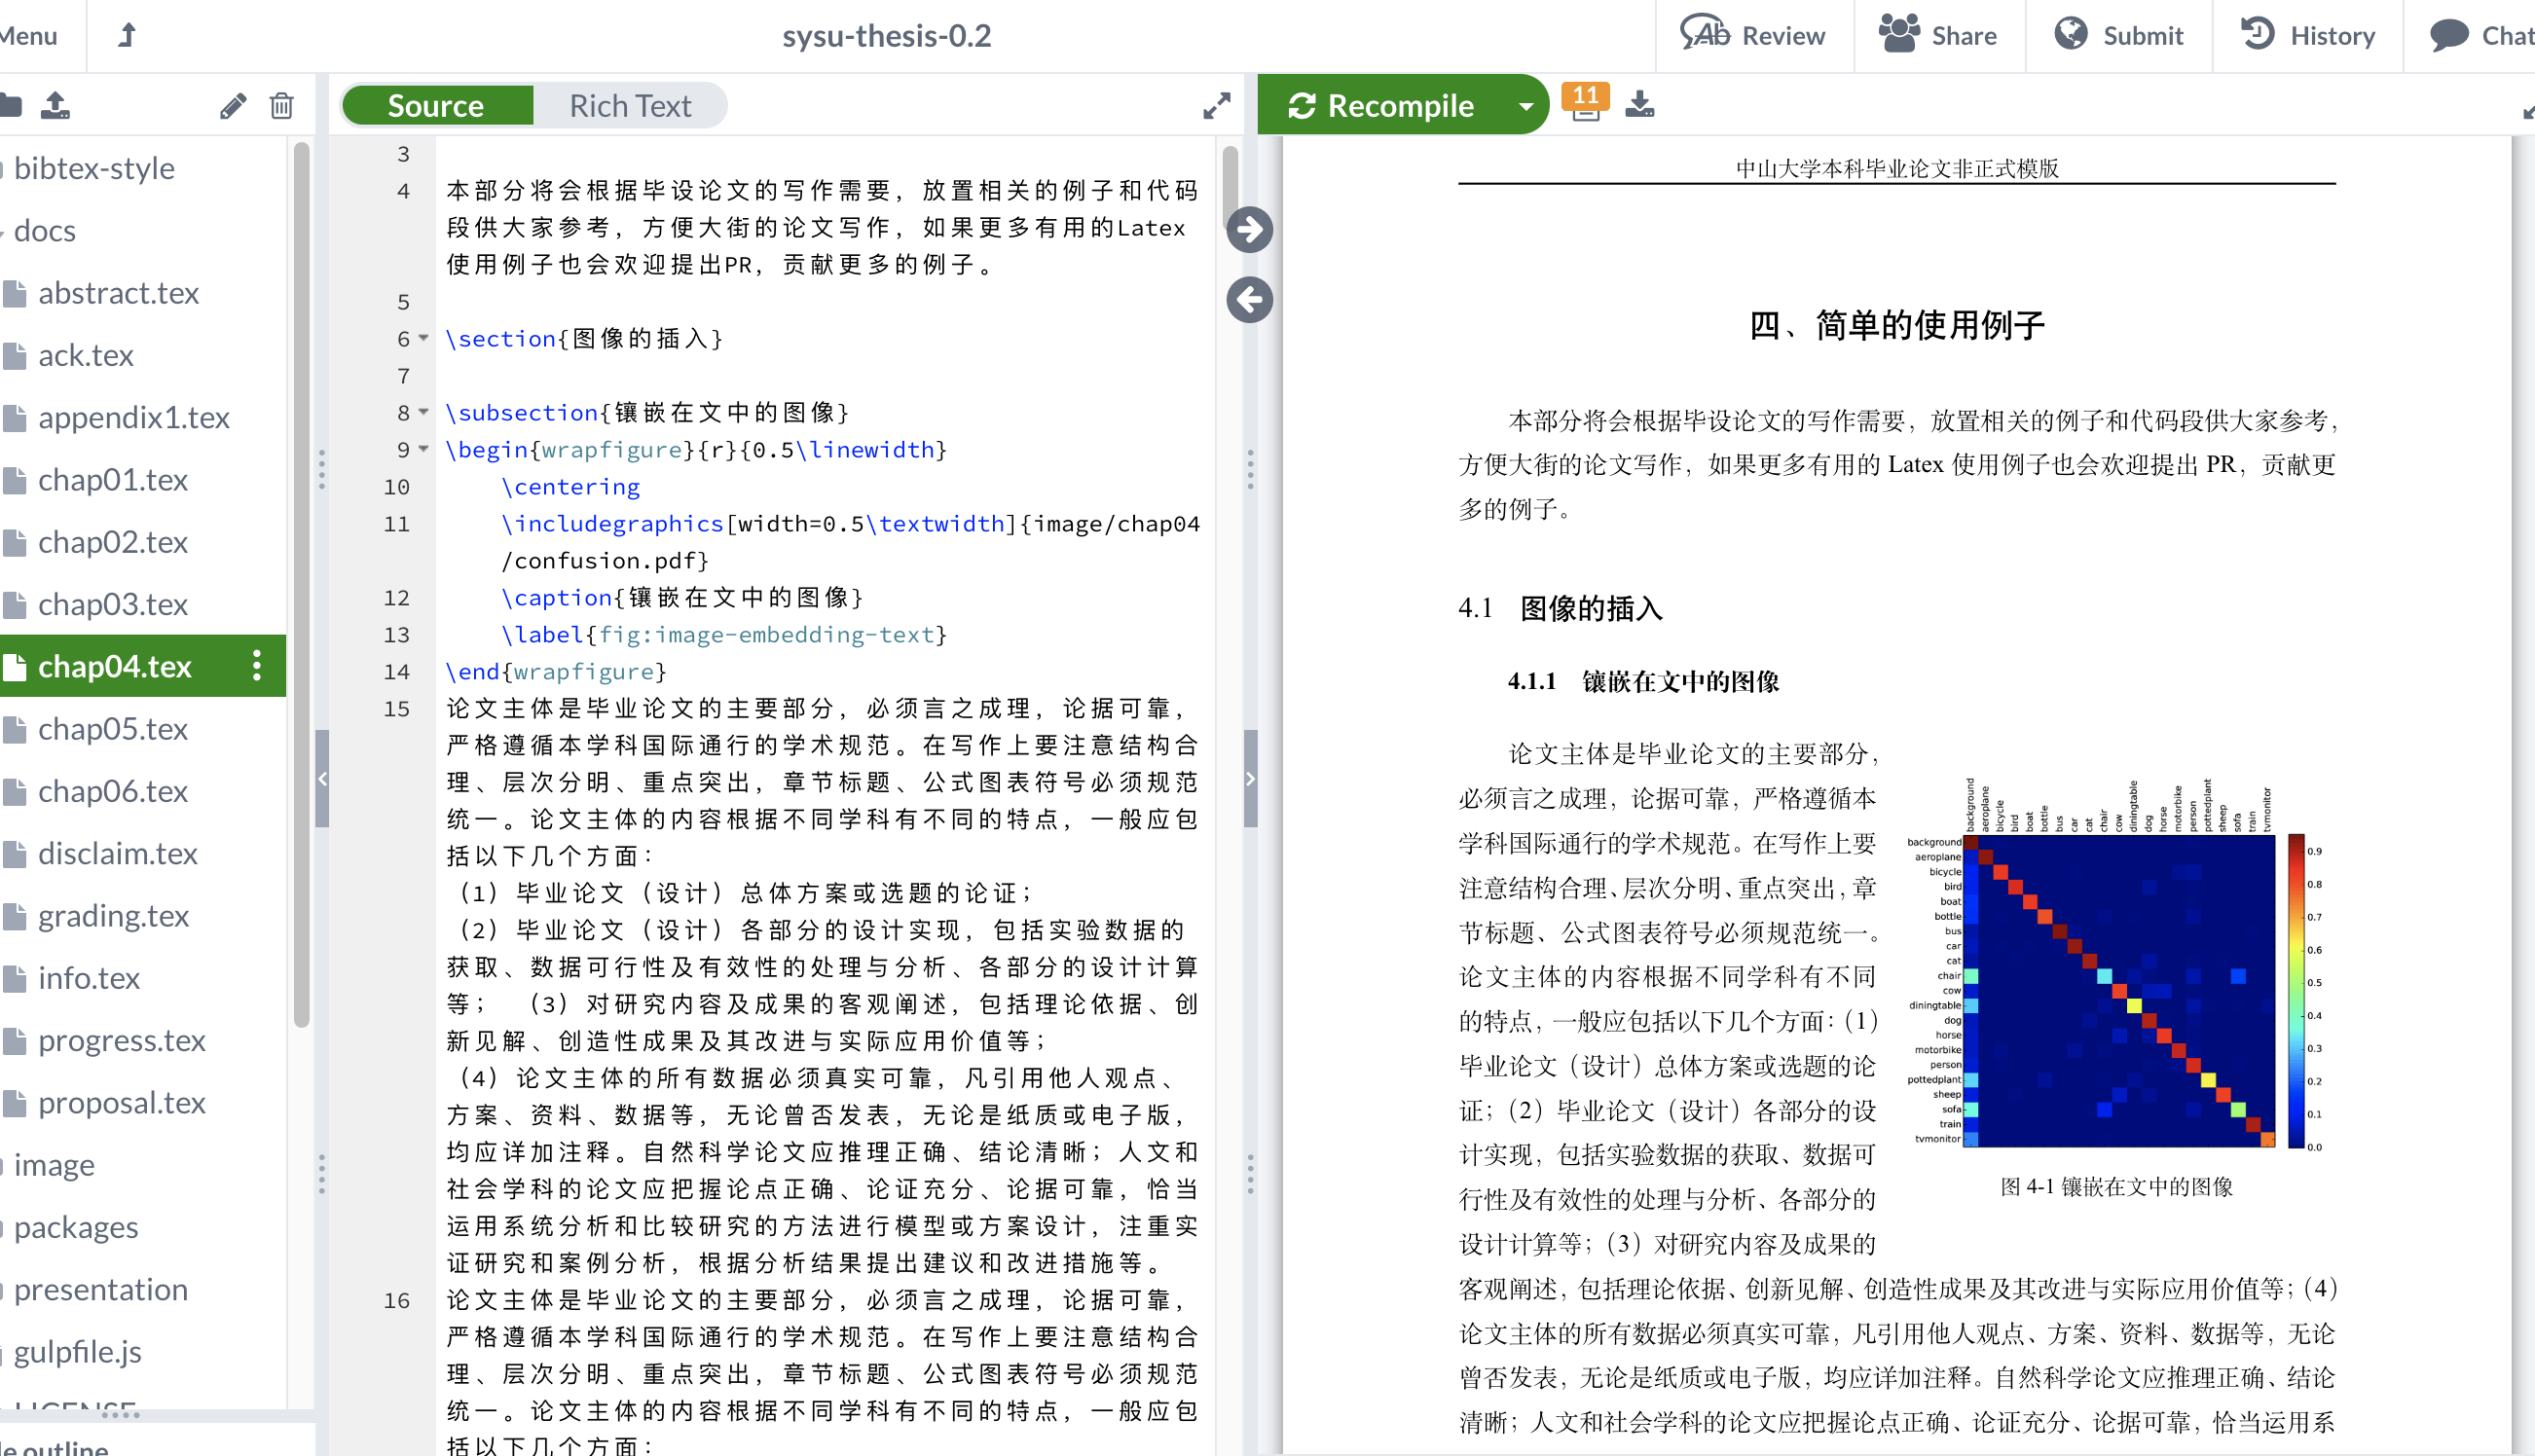
\includegraphics[width=0.9\textwidth]{image/chap03/overleaf-example.jpg}
% 	\caption{Overleaf使用例子}
% 	\label{fig:overleaf-example}
% \end{figure}



%\section{编译环境配置}

% 编译环境配置相对来说比较简单,下载Tex Live2020并如同一般的程序一样安装即可。

% \subsection{编译环境配置:Window篇}

% 在\url{https://mirrors.tuna.tsinghua.edu.cn/CTAN/systems/texlive/Images/}上下载Tex Live2020并参考教程\footnote{可以参考\url{https://zhuanlan.zhihu.com/p/58811994}}安装即可。

% \subsection{编译环境配置:Linux篇}

% 在\url{https://mirrors.tuna.tsinghua.edu.cn/CTAN/systems/texlive/Images/}上下载Tex Live2020并参考教程\footnote{可以参考\url{https://zhuanlan.zhihu.com/p/55894177}}安装即可。


% \subsection{编译环境配置:MacOS篇}

% 在MacOS上配置Latex的环境,这里我们使用的是MacTex。

% \begin{enumerate}
% 	\item \url{https://www.tug.org/mactex/}下载MacTex安装。
% 	\item 安装步骤:不详细展开,按照图形界面点击即可, 傻瓜式安装。
% \end{enumerate}

% TIPS:MacTex文件比较大,有2G多,介意的话可以选择MacTex\_Basic包,只有100M以内,但是如果安装MacTex\_Basic,后期可能会遇到各种缺包的问题。


% 安装完成之后,可以简单测试一下安装是否成功。如可以查看Texshop应用是否安装好,或者在命令行测试一下\texttt{xelatex}命令是否可用。

%\section{写作环境配置}

% 不同的写作工具对应不同的写作环境。这里我们给出几个工具的配置例子以供参考。

% \subsection{模板编译流程}

% 由于\LaTeX 的限制,本模板需要经过四次编译才能生成完整的论文:

% \begin{enumerate}
% 	\item 先使用xelatex编译一次
% 	\item 再使用bibtex编译一次
% 	\item 然后使用xelatex编译两次
% \end{enumerate}

% 本编译流程已经写在Makefile中,修改模板源码后只需要执行\texttt{make pdf}即可按照该流程进行编译并生成最终的pdf。



% \subsection{写作环境配置:Visual Studio Code}

% Visual Studio Code是微软公司推出的轻量代码编辑器,我们可以做一些简单的配置,便可以用该编辑器修改我们的\LaTeX 模板,并实现一键编译。

% \begin{enumerate}
% 	\item 安装 Visual Studio Code。
% 	\item 安装 LaTeX Workshop 插件。
% \end{enumerate}

% 本项目的\texttt{.vscode/setting.json}下已经包含了与前面所述编译流程相同的配置。正常配置下,每次修改模板源码后按下保存(Ctrl+S),就能够自动进行编译产生pdf。效果图如\autoref{fig:vscode-example}所示。


% \begin{figure}[h]
% 	\centering
% 	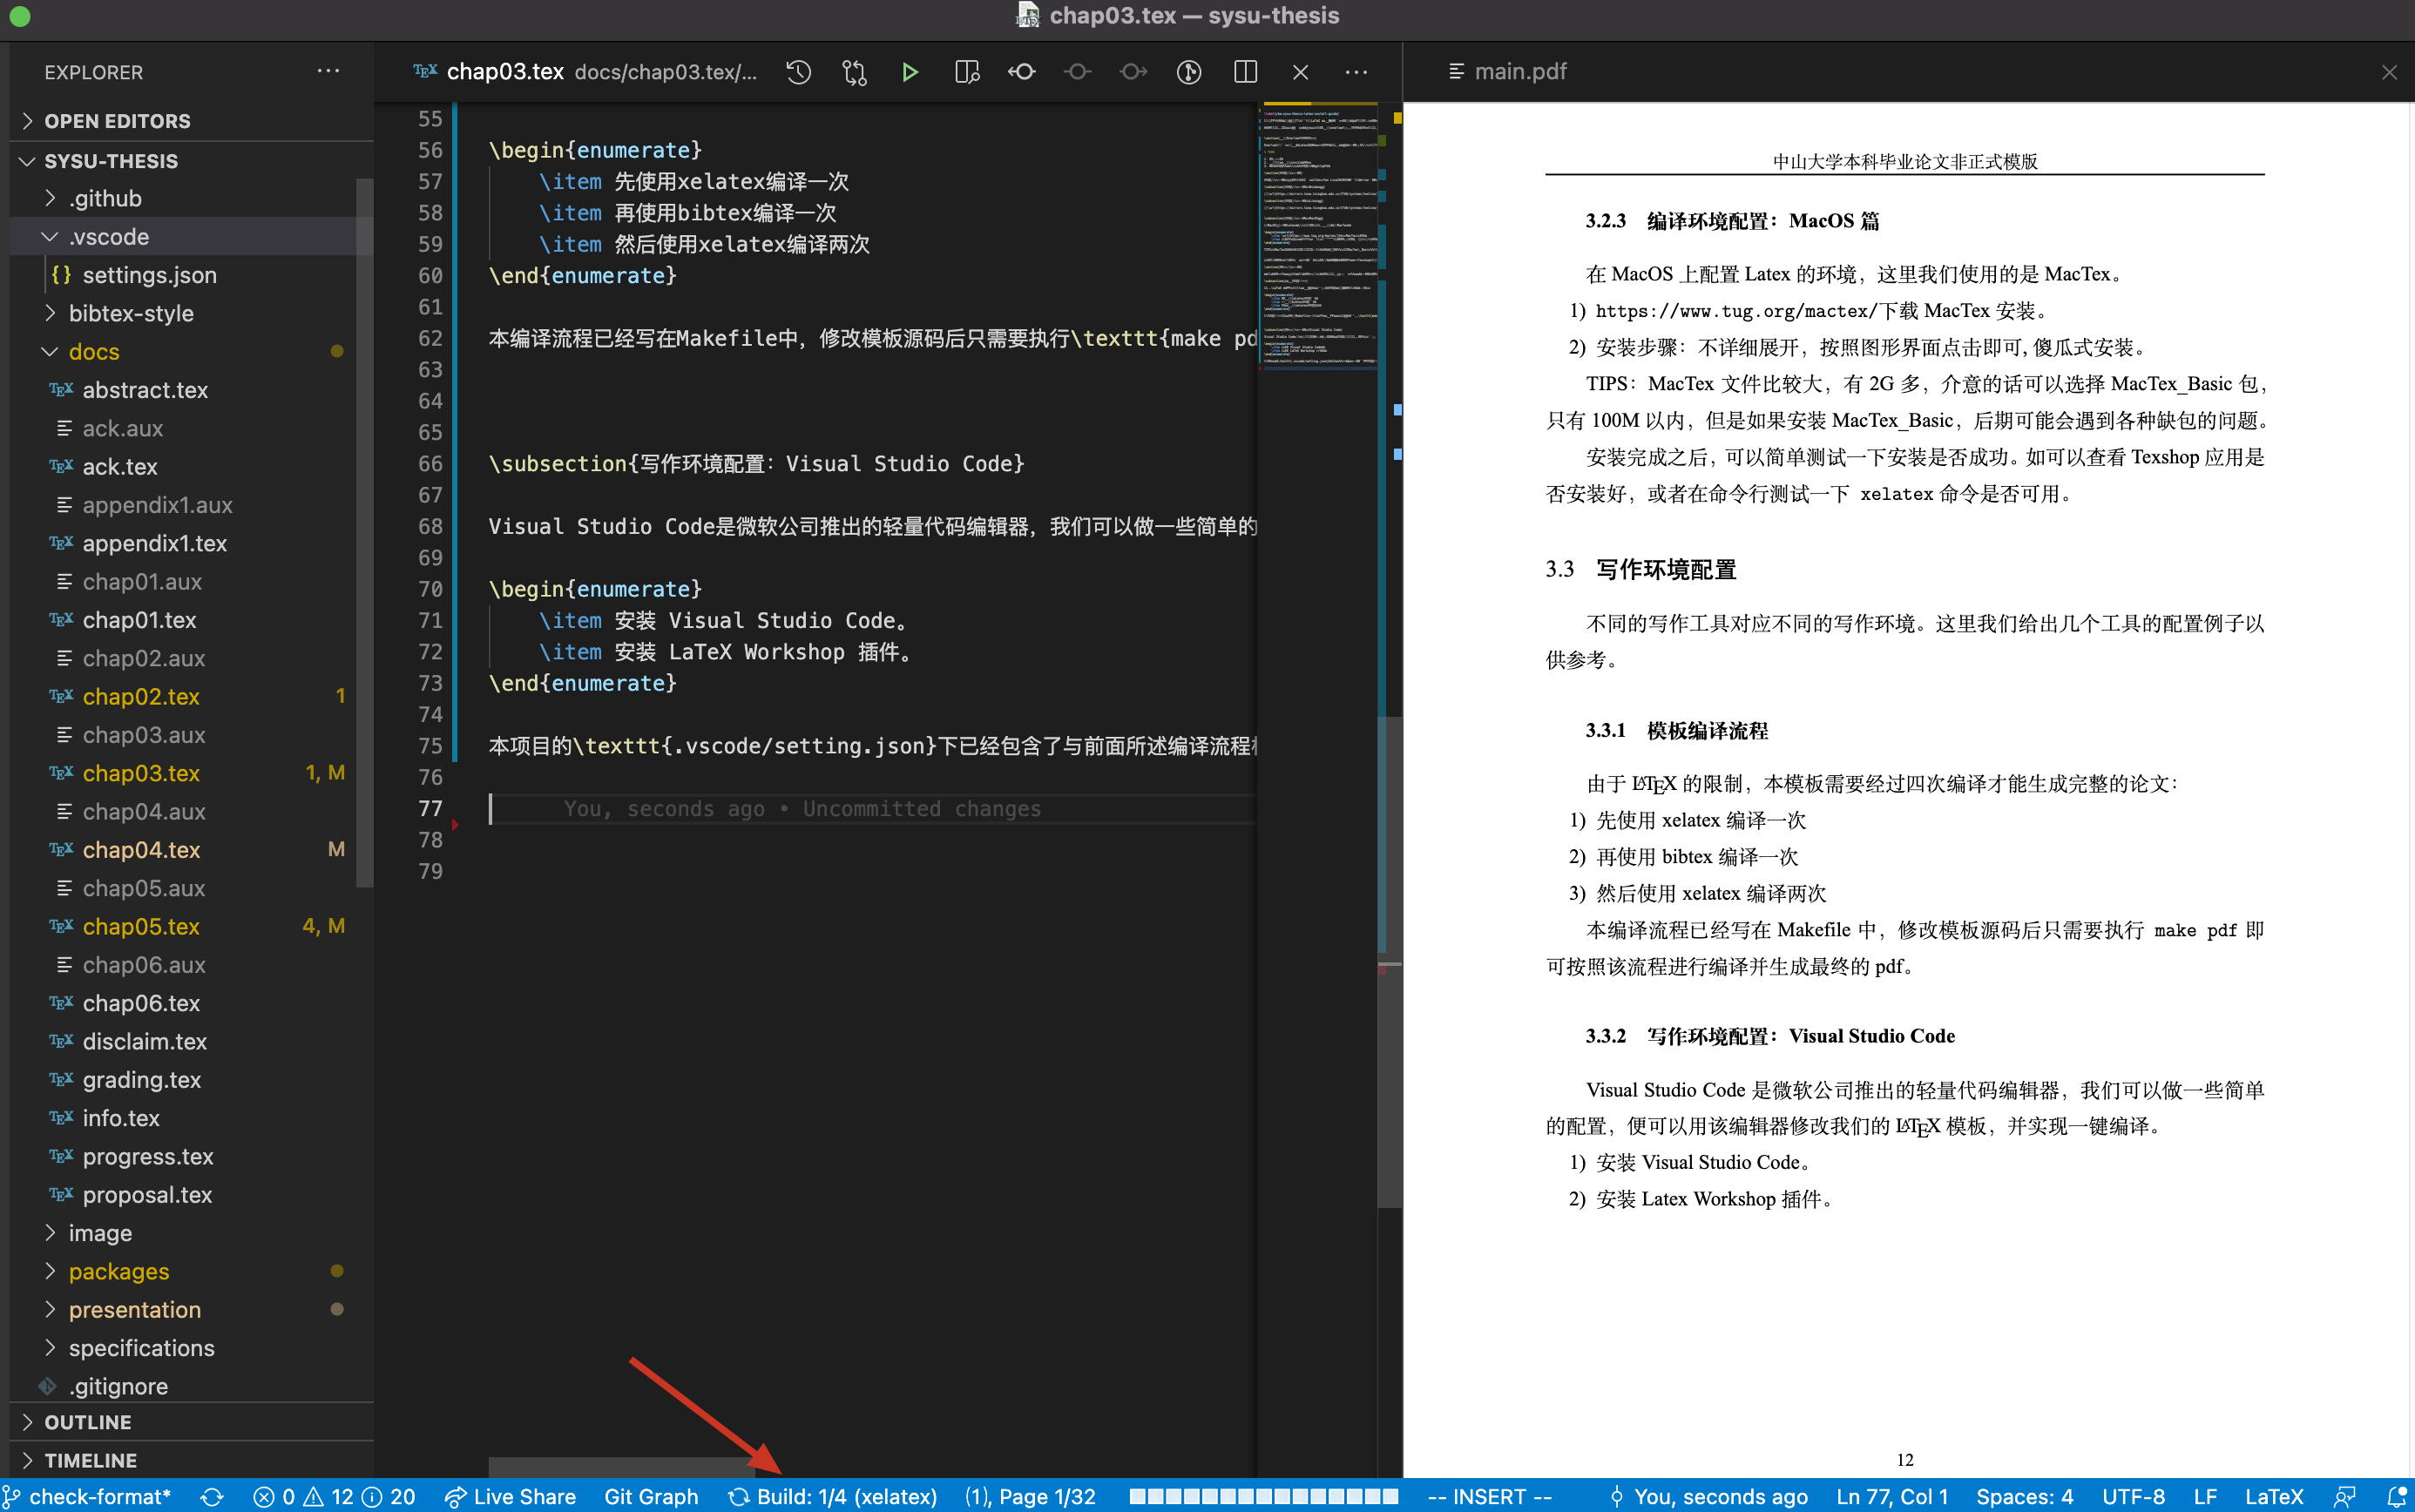
\includegraphics[width=\linewidth]{image/chap03/vscode-example.png}
% 	\caption{vscode配置好后的样例}
% 	\label{fig:vscode-example}
% \end{figure}


%\section{如何开始写毕业论文(设计)}

% 首先将所有个人信息,包括学号、姓名、专业、论文题目等,在\texttt{./docs/info.tex}中逐项进行更新。

% 然后我们再编辑\texttt{./docs/abstract.tex}补充论文摘要。

% 到了论文主体部分,我们可以自行编辑\texttt{./docs/chap01.tex},\texttt{./docs/chap02.tex}等文件进行编辑。如果章数不够,可以自行修改\texttt{main.tex}增加新的章节。

% 当论文主体编写完成后,我们再编辑\texttt{./docs/ack.tex}作为论文致谢。


% 首先将个人信息写到\texttt{./docs/info.tex}中。